%%%%%%%%%%%%%%%%%%%%%%%%%%%%%%%%%%%%%%%%%%%%%%%%%%%%%%%%%%%%%%%%%%%%%%%%%%%%%%%%%
% Introducción
%%%%%%%%%%%%%%%%%%%%%%%%%%%%%%%%%%%%%%%%%%%%%%%%%%%%%%%%%%%%%%%%%%%%%%%%%%%%%%%%%

\chapter{Estado del arte} % (fold)
\label{sec:EstadoDelArte}

    %%% Más cosas por aquí estaría bien, primero hay que entender que es Estado del Arte :)

    \section{Raspberry Pi} % (fold)
    \label{sec:RaspberryPi}

        \subsection{¿Qué es Raspberry Pi?} % (fold)
        \label{sub:QueEsRaspberryPi}

            ``Es un ordenador del tamaño de una tarjeta de crédito. Consta de una placa base sobre la que se monta un
            procesador, un chip gráfico y memoria RAM. Fue lanzado en 2006 por la Fundación Raspberry Pi con el objeto
            de estimular la enseñanza de informática en las escuelas de todo el mundo.''

            \begin{flushright}
                (El Confidencial, 22 de Noviembre de 2013. \cite{confidencial_raspberry})
            \end{flushright}

            Se ha vuelto un producto tan popular que se vende para todo tipo de usos, desde centros
            multimedia\cite{centro_multimedia_raspberry_pi} a espejos inteligentes\cite{espejo_raspberry_pi}, o este
            mismo proyecto.

        % subsection ¿Qué es Raspberry Pi? (end)

        \subsection{Modelos} % (fold)
        \label{sub:ModelosRaspberryPi}

            En sus ocho años de existencia, la Fundación Raspberry Pi ha lanzado cinco modelos de la Raspberry Pi, con
            diferentes variaciones. En la siguiente tabla se detallan alguno de los detalles de estos modelos:

            \begin{figure}[ht]
                \centering
                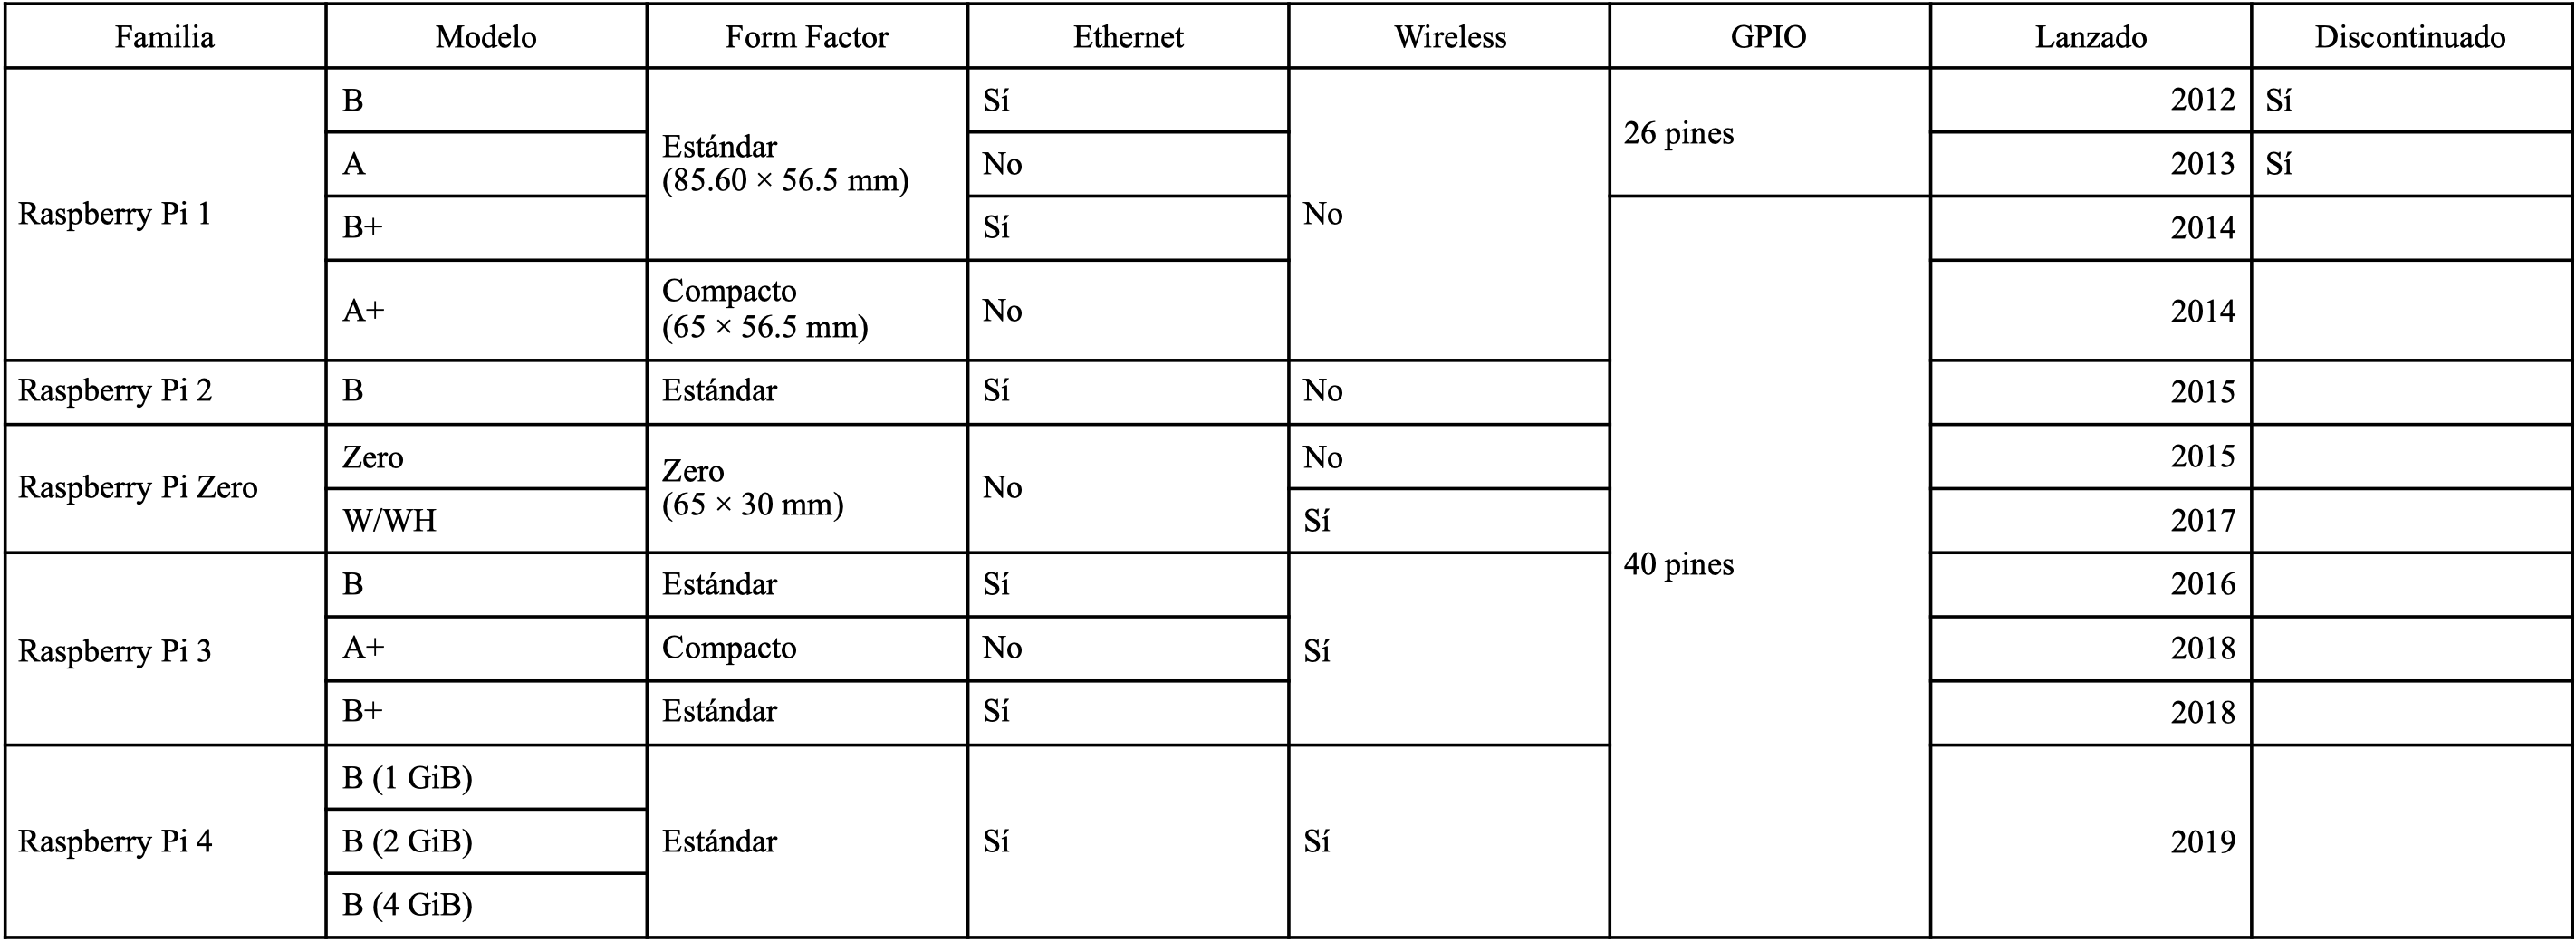
\includegraphics[width=\textwidth]{imagenes/tabla_modelos_raspberry_pi.png}
                \caption{Tabla modelos de Raspberry Pi\cite{raspberry_pi_wikipedia_en}}
            \end{figure}

        % subsection Modelos (end)

        \subsection{Hardware} % (fold)
        \label{sub:HardwareRaspberryPi}

            La Raspberry Pi 3B utilizada en este proyecto tiene el siguiente hardware\cite{raspberry_pi_hardware}:

            \begin{itemize}
                \item \textbf{Procesador:} Broadcom BCM2837 de cuatro núcleos con arquitectura ARM Cortex A53 (ARMv8) a
                1.2 GHz.
                \item \textbf{Memoria:} 1GB de memoria LPDDR2
                \item \textbf{GPU:} Broadcom VideoCore IV a 250 MHz
                \item \textbf{USB:} Cuatro puertos USB 2.0.
                \item \textbf{GPIO:} Hay 40 pines de GPIO (General Purpose Input/Output). Estos pines funcionan a 3.3V.
                \item \textbf{Internet:} Ethernet 10/100 Mbit/s y WiFi 802.11 b/g/n
            \end{itemize}

        % subsection Hardware (end)

    % section Raspberry Pi (end)
    \newpage
    \section{Opciones actuales en el mercado} % (fold)
    \label{sec:OpcionesActualesEnElMercado}

        Son múltiples las baterías electrónicas a la venta. Una búsqueda rápida en Thomann\cite{thomann_baterias} nos
        muestra una gran variedad de baterías electrónicas en un amplío rango de precios, desde los 109\euro{} hasta los
        8.398\euro{}.

        \begin{figure}[ht]
            \centering
            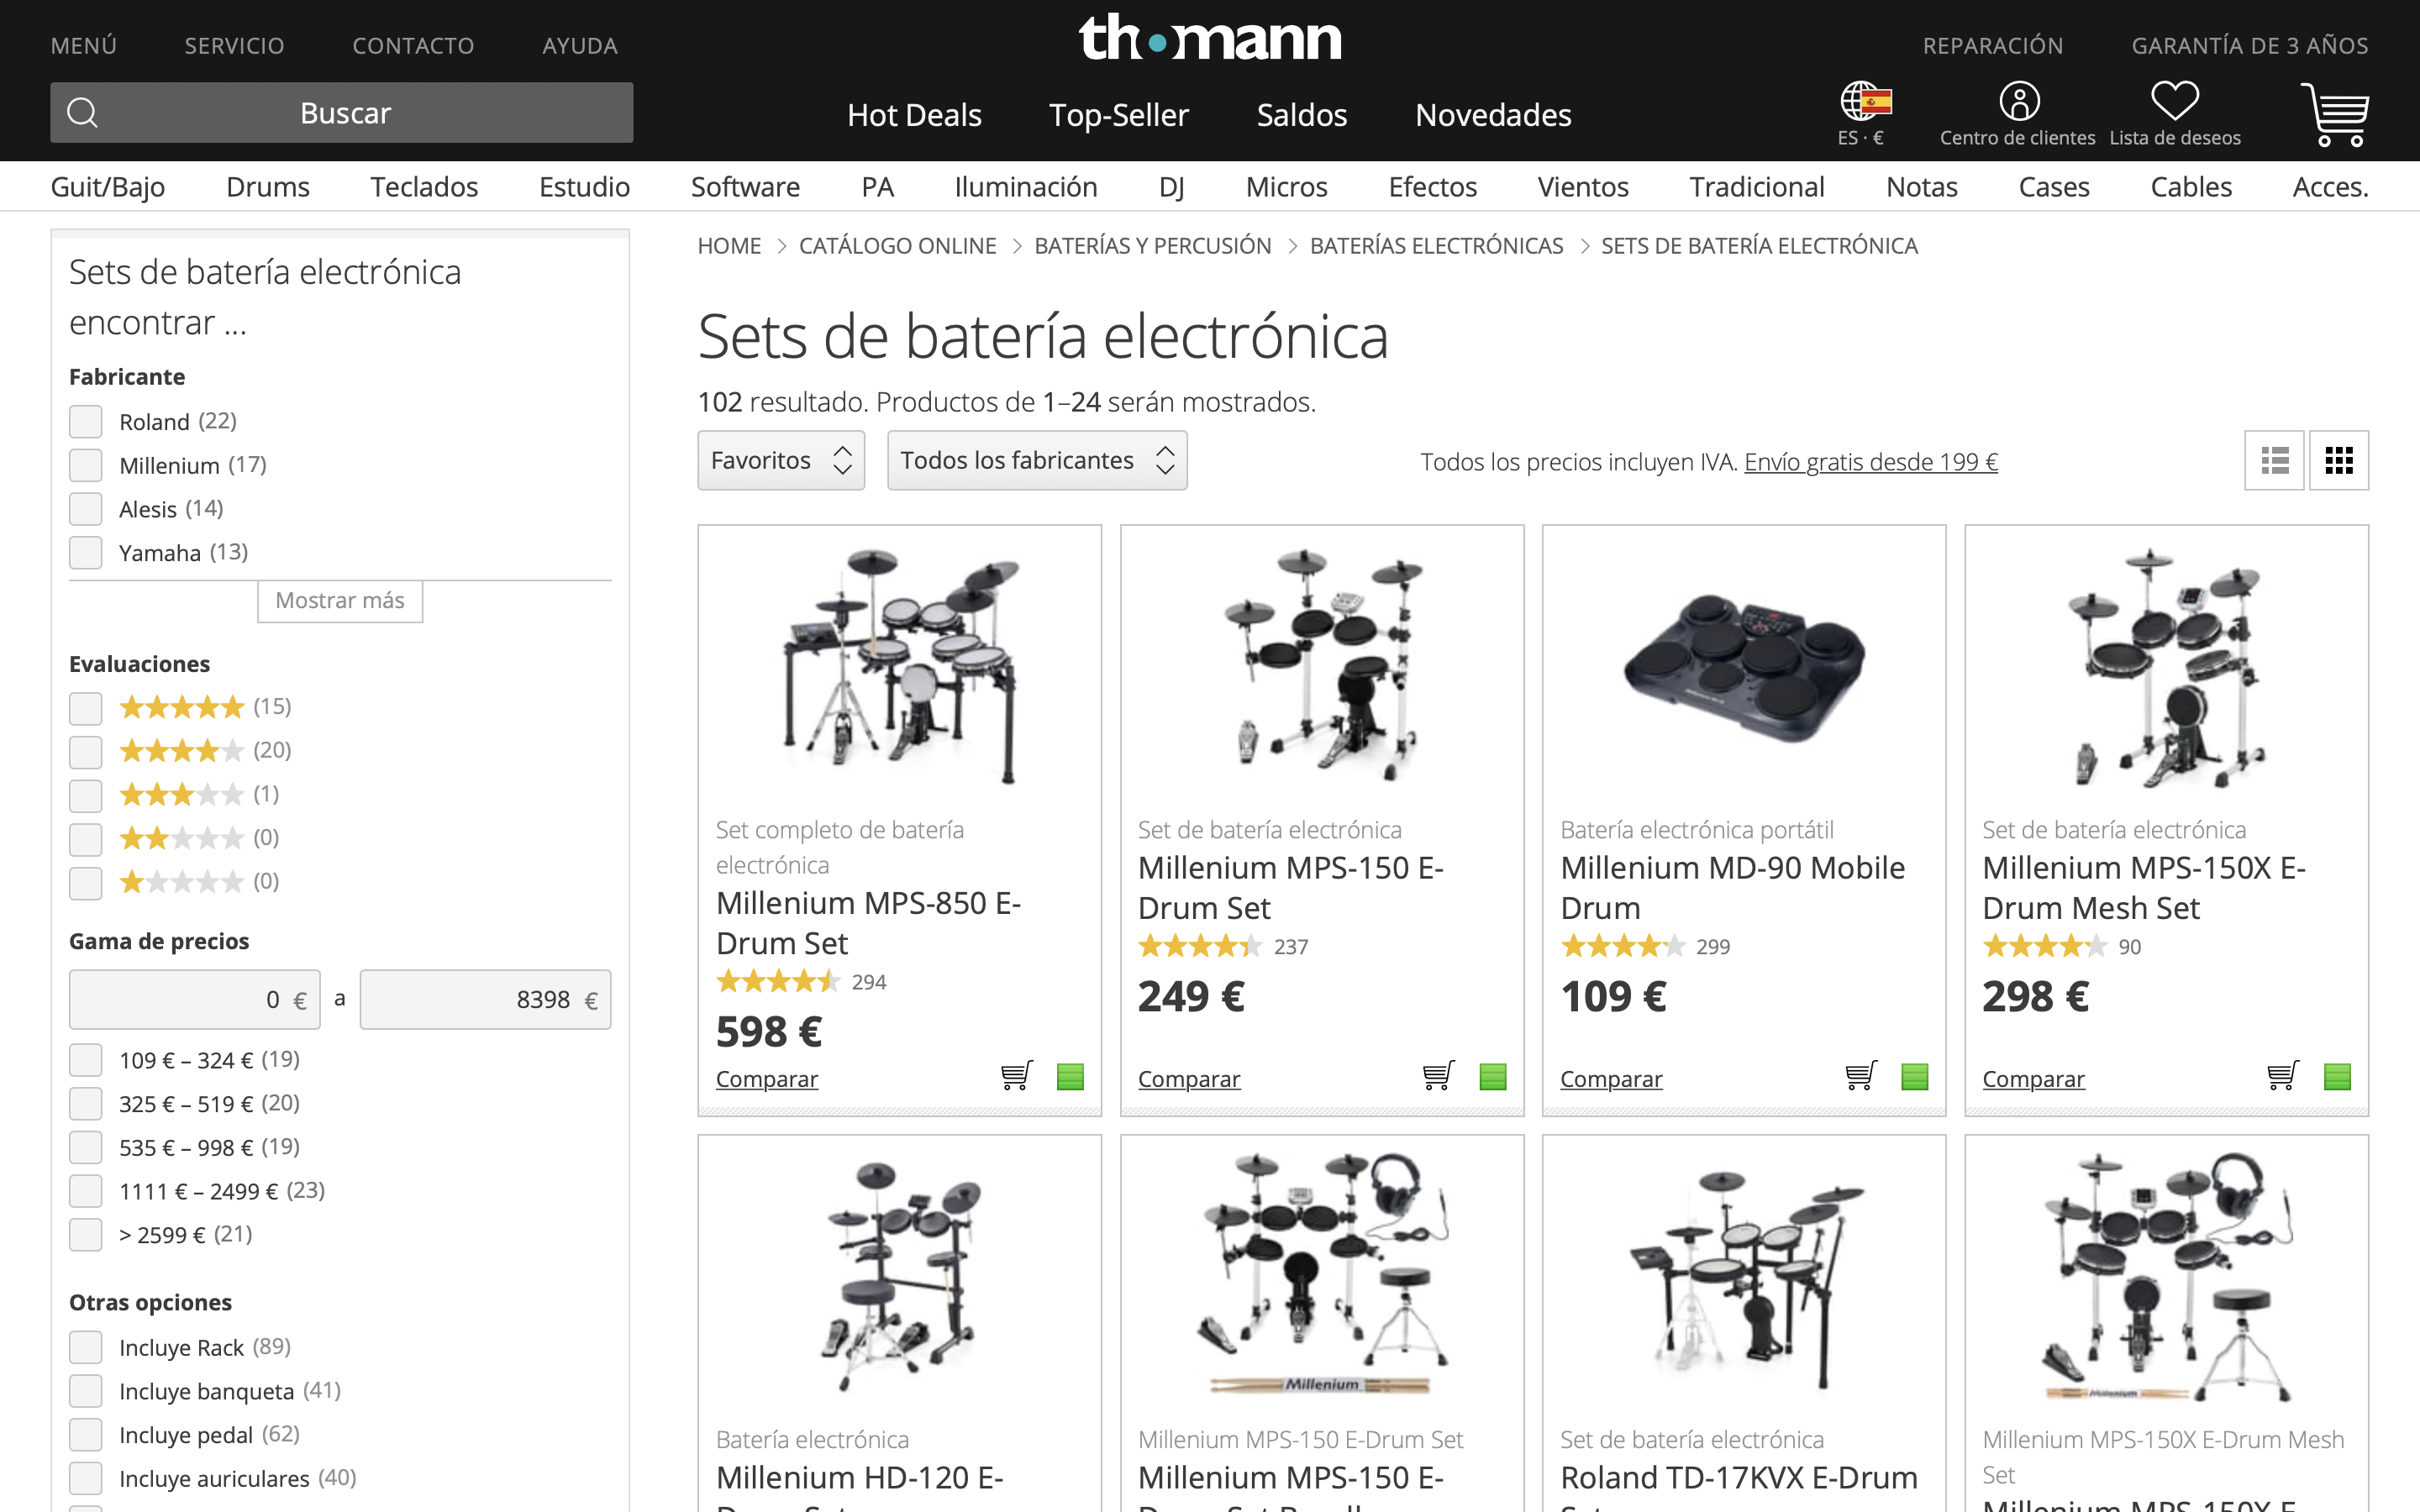
\includegraphics[width=\textwidth]{thomann_baterias}
            \caption{Resultados de la búsqueda de baterías electrónicas en Thomann}
        \end{figure}

        En el terreno del código abierto, %%%%%%%%%%%%%% cosas

    % section Opciones actuales en el mercado (end)

    \section{Propuesta} % (fold)
    \label{sec:Propuesta}

        La propuesta que se presenta es un crear un programa de código abierto para que cualquier persona con unos
        conocimiento medios de informática pueda montar su propia batería electrónica en casa.

        Para completar con éxito el objetivo de este proyecto, los puntos más importantes serán:
        \begin{itemize}
            \item Reproducción del sonido con el menor delay posible.
            \item Reproducción de varios sonidos al mismo tiempo.
            %%%%%%%%%%%%%%%%%%%%%%%%%%%%%%%%%%%%%%%%%%%%%%%%%%%%%%
        \end{itemize}

    % section Propuesta (end)

% chapter Estado del arte (end)
